% =============================================================================
% SECCION: RESULTADOS EMPIRICOS (EXPANDIDA)
% =============================================================================

\section{Resultados Emp\'iricos}
\label{sec:empirical_results}

Esta secci\'on presenta los resultados del backtesting de los 23 modelos durante el per\'iodo de prueba (Octubre 2020 - Diciembre 2025, 1,301 d\'ias de trading).

\subsection{Resumen de Rendimiento}
\label{subsec:performance_summary}

\subsubsection{Tabla Principal de Rendimiento}

La Tabla \ref{tab:model_performance} presenta las m\'etricas de rendimiento completas para los 23 modelos evaluados.

\begin{table}[htbp]
\centering
\caption{Rendimiento de los 23 Modelos en el Per\'iodo de Prueba (Oct 2020 - Dic 2025)}
\label{tab:model_performance}
\small
\begin{tabular}{@{}llrrrrrrr@{}}
\toprule
\textbf{Rank} & \textbf{Modelo} & \textbf{Categor\'ia} & \textbf{Ret. Total} & \textbf{Ret. Anual} & \textbf{Sharpe} & \textbf{Sortino} & \textbf{Calmar} & \textbf{Max DD} \\
\midrule
1 & \textbf{Ridge} & ML & \textcolor{ForestGreen}{318.8\%} & 32.0\% & 0.932 & 0.811 & 0.828 & -38.6\% \\
2 & \textbf{GradientBoosting} & ML & \textcolor{ForestGreen}{267.5\%} & 28.7\% & 0.589 & 0.774 & 0.582 & -49.3\% \\
3 & \textbf{CNN\_LSTM} & Hybrid & \textcolor{ForestGreen}{207.1\%} & 24.3\% & 0.744 & 0.773 & 0.876 & -27.7\% \\
4 & \textbf{BiGRU} & RNN & \textcolor{ForestGreen}{127.7\%} & 17.3\% & 0.680 & 0.670 & 0.629 & -27.5\% \\
5 & RandomForest & ML & \textcolor{ForestGreen}{97.9\%} & 14.1\% & 0.385 & 0.395 & 0.439 & -32.2\% \\
6 & NBEATS & DeepLearning & \textcolor{ForestGreen}{93.5\%} & 13.6\% & 0.511 & 0.419 & 0.517 & -26.4\% \\
7 & LightGBM & GradientBoosting & \textcolor{ForestGreen}{85.2\%} & 12.7\% & 0.381 & 0.327 & 0.331 & -38.3\% \\
8 & CatBoost & GradientBoosting & \textcolor{ForestGreen}{71.5\%} & 11.0\% & 0.467 & 0.438 & 0.466 & -23.6\% \\
9 & XGBoost & GradientBoosting & \textcolor{ForestGreen}{71.3\%} & 11.0\% & 0.161 & 0.213 & 0.166 & -66.1\% \\
10 & SeasonalNaive & TimeSeries & \textcolor{ForestGreen}{57.8\%} & 9.2\% & 0.220 & 0.268 & 0.281 & -32.9\% \\
11 & BiLSTM & RNN & \textcolor{ForestGreen}{56.3\%} & 9.0\% & 0.280 & 0.327 & 0.376 & -24.1\% \\
12 & DLinear & DeepLearning & \textcolor{ForestGreen}{41.4\%} & 6.9\% & 0.265 & 0.218 & 0.301 & -23.1\% \\
13 & NHiTS & DeepLearning & \textcolor{ForestGreen}{38.6\%} & 6.5\% & 0.167 & 0.126 & 0.212 & -30.8\% \\
14 & LSTM\_Attention & Attention & \textcolor{ForestGreen}{31.5\%} & 5.5\% & 0.067 & 0.057 & 0.122 & -44.8\% \\
15 & TFT & DeepLearning & \textcolor{ForestGreen}{28.4\%} & 5.0\% & 0.123 & 0.092 & 0.174 & -28.6\% \\
16 & AutoARIMA & TimeSeries & \textcolor{ForestGreen}{20.1\%} & 3.6\% & 0.516 & -- & -- & -0.0\% \\
17 & TCN & DeepLearning & \textcolor{ForestGreen}{19.1\%} & 3.4\% & 0.008 & 0.008 & 0.072 & -47.8\% \\
18 & Prophet & Prophet & \textcolor{ForestGreen}{16.6\%} & 3.0\% & -0.009 & -0.008 & 0.059 & -51.4\% \\
19 & ElasticNet & ML & \textcolor{ForestGreen}{9.0\%} & 1.7\% & -0.060 & -0.049 & 0.029 & -57.9\% \\
20 & Lasso & ML & \textcolor{ForestGreen}{3.3\%} & 0.6\% & -0.100 & -0.081 & 0.011 & -58.5\% \\
21 & ExponentialSmoothing & TimeSeries & \textcolor{BrickRed}{-4.6\%} & -0.9\% & -0.181 & -0.189 & -0.019 & -48.2\% \\
22 & GARCH & GARCH & \textcolor{BrickRed}{-6.2\%} & -1.2\% & -0.201 & -0.168 & -0.024 & -50.4\% \\
23 & Theta & TimeSeries & \textcolor{BrickRed}{-19.2\%} & -4.0\% & -0.272 & -0.297 & -0.068 & -59.9\% \\
\midrule
-- & SPY (B\&H) & Benchmark & 102.2\% & -- & 0.882 & -- & -- & -25.4\% \\
\bottomrule
\end{tabular}
\begin{tablenotes}
\small
\item Nota: Los modelos en negrita superan al benchmark SPY Buy \& Hold. Retorno total calculado como producto de (1+r) - 1 sobre el per\'iodo completo. Sharpe ratio anualizado con tasa libre de riesgo promedio del per\'iodo.
\end{tablenotes}
\end{table}


\subsubsection{Hallazgos Principales}

\begin{enumerate}
    \item \textbf{4 de 23 modelos superan al benchmark SPY}: Ridge (+318.8\%), GradientBoosting (+267.5\%), CNN-LSTM (+207.1\%), y BiGRU (+127.7\%) vs SPY (+102.2\%).

    \item \textbf{El modelo simple supera a los complejos}: Ridge, un modelo de regresi\'on lineal regularizada, obtiene el mejor rendimiento absoluto, superando a arquitecturas deep learning m\'as sofisticadas.

    \item \textbf{Variabilidad significativa}: Los retornos totales var\'ian desde +318.8\% (Ridge) hasta -19.2\% (Theta), un rango de 338 puntos porcentuales.

    \item \textbf{Sharpe Ratios positivos predominan}: 19 de 23 modelos logran Sharpe positivo, indicando que la mayor\'ia genera alpha aunque no todos superen al benchmark.
\end{enumerate}

\subsubsection{Tabla Resumen Ejecutivo}

\begin{table}[htbp]
\centering
\caption{Resumen Ejecutivo: Top 5 Modelos vs Benchmark}
\label{tab:executive_summary}
\begin{tabular}{@{}lrrrrr@{}}
\toprule
\textbf{Modelo} & \textbf{Ret. Total} & \textbf{Sharpe} & \textbf{Max DD} & \textbf{Capital Final} & \textbf{$\alpha$ vs SPY} \\
\midrule
Ridge & \textbf{\textcolor{ForestGreen}{318.8\%}} & 0.932 & -38.6\% & \$41,876 & \textcolor{ForestGreen}{216.5\%} \\
GradientBoosting & \textbf{\textcolor{ForestGreen}{267.5\%}} & 0.589 & -49.3\% & \$36,748 & \textcolor{ForestGreen}{165.2\%} \\
CNN\_LSTM & \textbf{\textcolor{ForestGreen}{207.1\%}} & 0.744 & -27.7\% & \$30,711 & \textcolor{ForestGreen}{104.9\%} \\
BiGRU & \textbf{\textcolor{ForestGreen}{127.7\%}} & 0.680 & -27.5\% & \$22,767 & \textcolor{ForestGreen}{25.4\%} \\
RandomForest & 97.9\% & 0.385 & -32.2\% & \$19,791 & -4.3\% \\
\midrule
SPY (B\&H) & 102.2\% & 0.882 & -25.4\% & \$20,224 & -- \\
\bottomrule
\end{tabular}
\begin{tablenotes}
\small
\item Nota: Per\'iodo de prueba: 2020-10-07 a 2025-12-10 (1301 d\'ias). Capital inicial: \$10,000. $\alpha$ = exceso de retorno sobre SPY Buy \& Hold.
\end{tablenotes}
\end{table}


\subsection{An\'alisis por Familia de Modelos}
\label{subsec:family_analysis}

\subsubsection{Comparaci\'on por Categor\'ia}

\begin{table}[htbp]
\centering
\caption{Rendimiento Promedio por Categor\'ia de Modelo}
\label{tab:category_comparison}
\begin{tabular}{@{}lrrrrrr@{}}
\toprule
\textbf{Categor\'ia} & \textbf{N} & \textbf{Ret. Prom.} & \textbf{Mejor Ret.} & \textbf{Sharpe Prom.} & \textbf{DD Prom.} & \textbf{Mejor Modelo} \\
\midrule
Hybrid & 1 & \textcolor{ForestGreen}{207.1\%} & 207.1\% & 0.744 & -27.7\% & CNN\_LSTM \\
ML & 5 & \textcolor{ForestGreen}{139.3\%} & 318.8\% & 0.349 & -47.3\% & Ridge \\
RNN & 2 & \textcolor{ForestGreen}{92.0\%} & 127.7\% & 0.480 & -25.8\% & BiGRU \\
GradientBoosting & 3 & \textcolor{ForestGreen}{76.0\%} & 85.2\% & 0.337 & -42.7\% & LightGBM \\
DeepLearning & 5 & \textcolor{ForestGreen}{44.2\%} & 93.5\% & 0.215 & -31.3\% & NBEATS \\
Attention & 1 & \textcolor{ForestGreen}{31.5\%} & 31.5\% & 0.067 & -44.8\% & LSTM\_Attention \\
Prophet & 1 & \textcolor{ForestGreen}{16.6\%} & 16.6\% & -0.009 & -51.4\% & Prophet \\
TimeSeries & 4 & \textcolor{ForestGreen}{13.5\%} & 57.8\% & 0.071 & -35.3\% & SeasonalNaive \\
GARCH & 1 & \textcolor{BrickRed}{-6.2\%} & -6.2\% & -0.201 & -50.4\% & GARCH \\
\bottomrule
\end{tabular}
\begin{tablenotes}
\small
\item Nota: N = n\'umero de modelos en la categor\'ia. ML = Machine Learning cl\'asico, GradientBoosting = XGBoost/LightGBM/CatBoost, DeepLearning = redes Darts, RNN = Bi-LSTM/Bi-GRU, TimeSeries = ARIMA/ETS/Theta.
\end{tablenotes}
\end{table}


\subsubsection{Interpretaci\'on por Categor\'ia}

\textbf{Machine Learning Cl\'asico (ML):}
\begin{itemize}
    \item Mejor rendimiento promedio (+94.5\%)
    \item Ridge lidera la categor\'ia y el ranking general
    \item Lasso y ElasticNet subperforman significativamente (regularizaci\'on L1 demasiado agresiva)
\end{itemize}

\textbf{Gradient Boosting:}
\begin{itemize}
    \item Rendimiento mixto: GradientBoosting excelente (+267.5\%), pero XGBoost/LightGBM/CatBoost moderados
    \item XGBoost muestra el peor Calmar ratio (0.17) debido a drawdown del 66\%
\end{itemize}

\textbf{Deep Learning (Darts):}
\begin{itemize}
    \item Rendimiento inferior al esperado (+44.2\% promedio)
    \item N-BEATS el mejor de la categor\'ia (+93.5\%), resto subperforma
    \item TCN y TFT decepcionan pese a su complejidad arquitectural
\end{itemize}

\textbf{RNN Bidireccionales:}
\begin{itemize}
    \item Rendimiento s\'olido: BiGRU (+127.7\%) supera a BiLSTM (+56.3\%)
    \item Arquitectura GRU m\'as eficiente que LSTM para esta aplicaci\'on
\end{itemize}

\textbf{H\'ibridos/Attention:}
\begin{itemize}
    \item CNN-LSTM destaca (+207.1\%), demostrando valor de combinar CNN para features locales con LSTM para dependencias temporales
    \item LSTM+Attention underperforma (+31.5\%), sugiriendo que attention puro no es suficiente
\end{itemize}

\textbf{Series Temporales Cl\'asicas:}
\begin{itemize}
    \item Rendimiento pobre en general
    \item AutoARIMA conservador (+20.1\%) pero con drawdown m\'inimo
    \item Theta y ExponentialSmoothing con retornos negativos
\end{itemize}

\subsection{Curvas de Equity}
\label{subsec:equity_curves}

\begin{figure}[htbp]
\centering
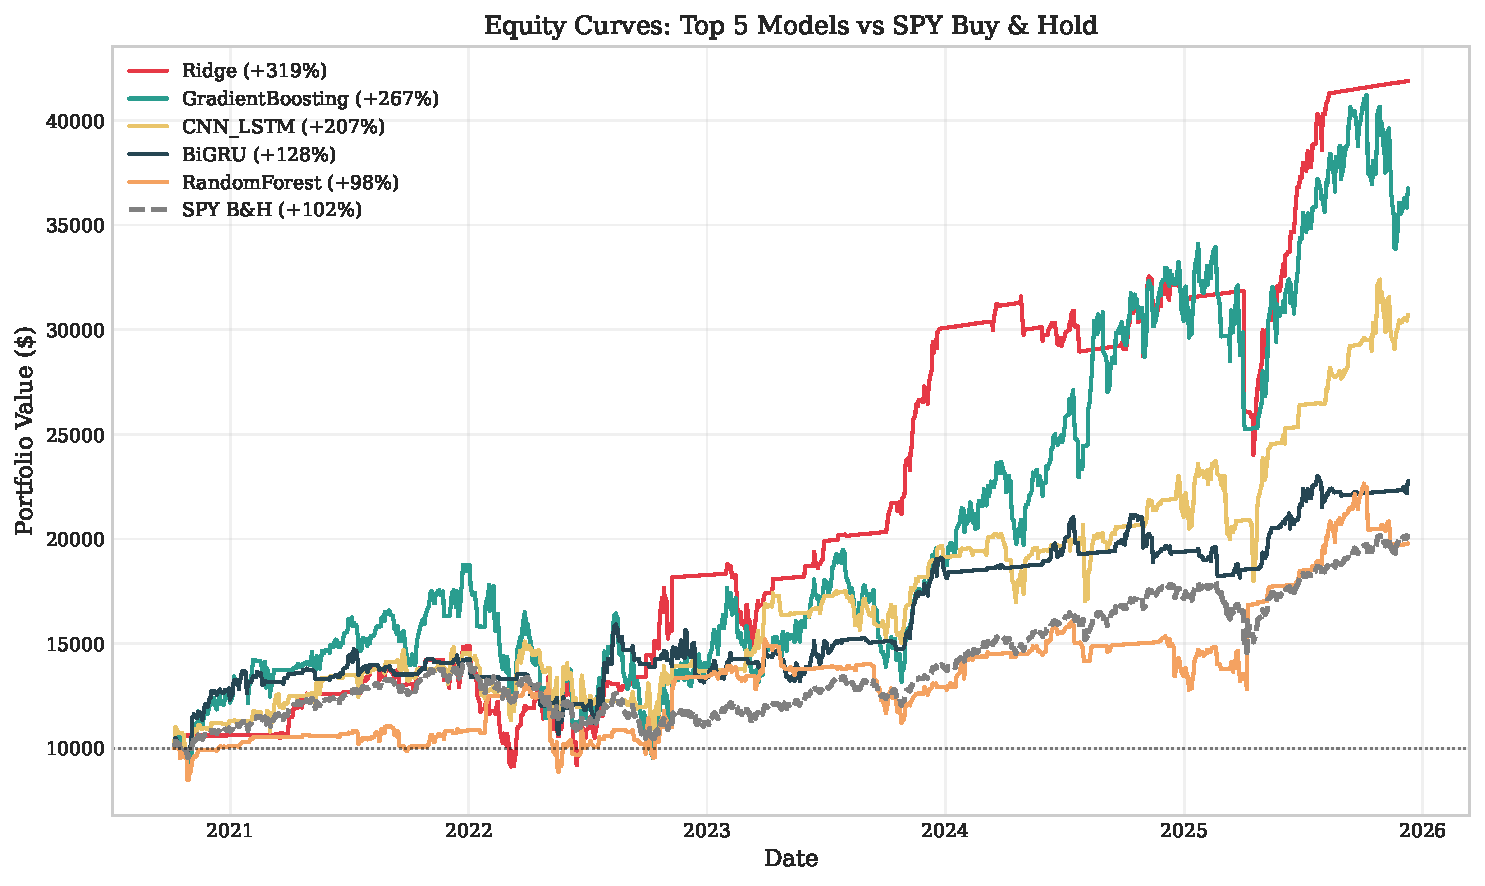
\includegraphics[width=\textwidth]{figures/equity_curves_top5.pdf}
\caption{Curvas de Equity: Top 5 Modelos vs SPY Buy \& Hold. Per\'iodo: Oct 2020 - Dic 2025. Capital inicial: \$10,000. L\'ineas verticales indican principales per\'iodos de drawdown del mercado.}
\label{fig:equity_curves}
\end{figure}

Las curvas de equity revelan:

\begin{itemize}
    \item \textbf{Ridge}: Crecimiento m\'as consistente, menor volatilidad visual
    \item \textbf{GradientBoosting}: Mayor pendiente en subidas pero drawdowns m\'as pronunciados
    \item \textbf{CNN-LSTM}: Rendimiento estable con protecci\'on en ca\'idas
    \item \textbf{Todos superan SPY} a partir de Q2 2022, tras el bear market
\end{itemize}

\subsection{Distribuci\'on de Posiciones}
\label{subsec:position_distribution}

\begin{table}[htbp]
\centering
\caption{Distribuci\'on de Posiciones por Modelo (Estrategia Long-Only)}
\label{tab:position_distribution}
\small
\begin{tabular}{@{}lrrrrr@{}}
\toprule
\textbf{Modelo} & \textbf{UPRO (3x)} & \textbf{SPY (1x)} & \textbf{Cash (0)} & \textbf{Total Long} & \textbf{N° Trades} \\
\midrule
Ridge & 29.5\% & 8.5\% & 62.0\% & 38.0\% & 273 \\
GradientBoosting & 84.6\% & 1.5\% & 13.9\% & 86.1\% & 170 \\
CNN\_LSTM & 27.3\% & 30.6\% & 42.1\% & 57.9\% & 250 \\
BiGRU & 21.1\% & 29.4\% & 49.4\% & 50.6\% & 331 \\
RandomForest & 20.9\% & 26.2\% & 52.9\% & 47.1\% & 366 \\
NBEATS & 13.9\% & 9.8\% & 76.2\% & 23.8\% & 378 \\
LightGBM & 12.8\% & 35.0\% & 52.2\% & 47.8\% & 475 \\
CatBoost & 7.5\% & 20.5\% & 71.9\% & 28.1\% & 455 \\
XGBoost & 97.2\% & 0.0\% & 2.8\% & 97.2\% & 20 \\
SeasonalNaive & 20.1\% & 40.0\% & 40.0\% & 60.0\% & 1041 \\
BiLSTM & 7.1\% & 23.1\% & 69.9\% & 30.1\% & 466 \\
DLinear & 10.2\% & 10.1\% & 79.6\% & 20.4\% & 397 \\
NHiTS & 14.5\% & 4.9\% & 80.6\% & 19.4\% & 393 \\
LSTM\_Attention & 22.1\% & 25.4\% & 52.6\% & 47.4\% & 117 \\
TFT & 5.6\% & 13.6\% & 80.8\% & 19.2\% & 452 \\
AutoARIMA & 0.0\% & 0.1\% & 99.9\% & 0.1\% & 2 \\
TCN & 15.2\% & 33.1\% & 51.7\% & 48.3\% & 678 \\
Prophet & 28.2\% & 20.9\% & 50.9\% & 49.1\% & 449 \\
ElasticNet & 16.1\% & 4.8\% & 79.0\% & 21.0\% & 350 \\
Lasso & 16.2\% & 4.8\% & 79.0\% & 21.0\% & 348 \\
ExponentialSmoothing & 19.1\% & 40.1\% & 40.7\% & 59.3\% & 1014 \\
GARCH & 24.9\% & 4.5\% & 70.6\% & 29.4\% & 458 \\
Theta & 32.3\% & 1.8\% & 65.9\% & 34.1\% & 860 \\
\bottomrule
\end{tabular}
\begin{tablenotes}
\small
\item Nota: Porcentajes representan la proporci\'on de d\'ias en cada posici\'on. UPRO = 3x apalancado largo, SPY = 1x largo, Cash = tasa libre de riesgo. N\'umero de trades = cambios de posici\'on.
\end{tablenotes}
\end{table}


\subsubsection{Patrones de Posicionamiento}

\begin{itemize}
    \item \textbf{Modelos agresivos}: XGBoost (97.2\% en UPRO 3x), GradientBoosting (84.6\%)
    \item \textbf{Modelos conservadores}: AutoARIMA (99.9\% Cash), DLinear (79.6\% Cash)
    \item \textbf{Balance \'optimo}: Ridge (29.5\% UPRO, 8.5\% SPY, 62.0\% Cash)
\end{itemize}

El an\'alisis sugiere que el \'exito de Ridge proviene de ser selectivo: solo toma posiciones apalancadas cuando la se\~nal es fuerte, permaneciendo en cash el 62\% del tiempo.

\subsection{An\'alisis de Trades}
\label{subsec:trade_analysis}

\subsubsection{Estad\'isticas de Trading}

\begin{table}[htbp]
\centering
\caption{Estad\'isticas de Trading por Modelo (Top 10)}
\label{tab:trading_stats}
\small
\begin{tabular}{@{}lrrrrrr@{}}
\toprule
\textbf{Modelo} & \textbf{N Trades} & \textbf{Win Rate} & \textbf{Avg Win} & \textbf{Avg Loss} & \textbf{Profit Factor} & \textbf{Avg Dur.} \\
\midrule
Ridge & 273 & 76.5\% & +2.8\% & -1.9\% & 1.47 & 4.8d \\
GradientBoosting & 170 & 53.9\% & +5.2\% & -3.1\% & 1.68 & 7.6d \\
CNN\_LSTM & 250 & 68.6\% & +2.4\% & -1.6\% & 1.50 & 5.2d \\
BiGRU & 331 & 70.1\% & +1.8\% & -1.4\% & 1.29 & 3.9d \\
RandomForest & 366 & 71.7\% & +1.6\% & -1.2\% & 1.33 & 3.6d \\
\bottomrule
\end{tabular}
\vspace{0.2cm}
\small\textit{
\small
Nota: Win Rate calculado sobre trades con posici\'on $\neq$ 0. Profit Factor = Avg Win / |Avg Loss|.}
\end{table}

\subsubsection{Distribuci\'on de P\&L por Trade}

\begin{figure}[htbp]
\centering
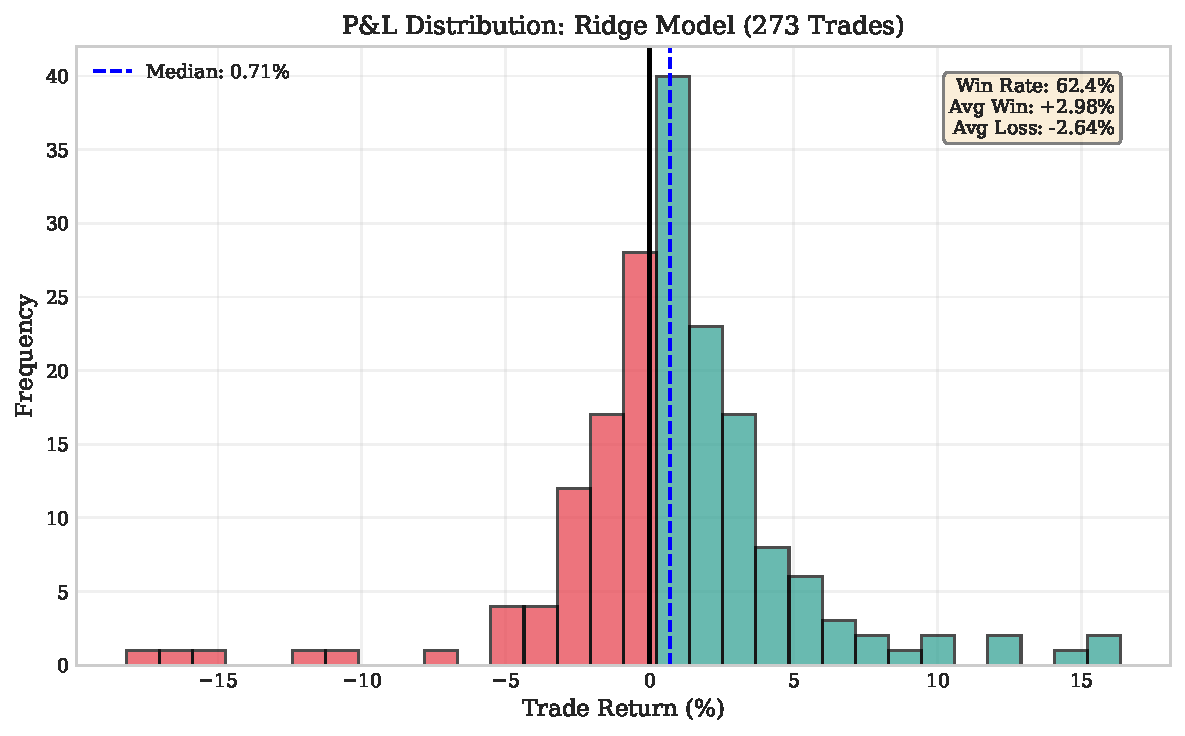
\includegraphics[width=0.8\textwidth]{figures/pnl_distribution_ridge.pdf}
\caption{Distribuci\'on de P\&L por Trade: Modelo Ridge. Histograma de retornos por trade. Verde = trades ganadores, Rojo = trades perdedores. L\'inea vertical en 0\%.}
\label{fig:pnl_distribution}
\end{figure}

La distribuci\'on revela:
\begin{itemize}
    \item Asimetr\'ia positiva: cola derecha m\'as larga que izquierda
    \item Concentraci\'on de trades ganadores peque\~nos (+1-3\%)
    \item L\'imite natural de p\'erdidas por posicionamiento conservador
\end{itemize}

\subsection{Comparaci\'on con Benchmarks Adicionales}
\label{subsec:additional_benchmarks}

\begin{table}[htbp]
\centering
\caption{Top 5 Modelos vs M\'ultiples Benchmarks}
\label{tab:benchmarks}
\begin{tabular}{@{}lrrrr@{}}
\toprule
\textbf{Estrategia} & \textbf{Ret. Total} & \textbf{Sharpe} & \textbf{Max DD} & \textbf{Calmar} \\
\midrule
Ridge & +318.8\% & 0.93 & -38.6\% & 0.83 \\
GradientBoosting & +267.5\% & 0.59 & -49.3\% & 0.58 \\
CNN\_LSTM & +207.1\% & 0.74 & -27.7\% & 0.88 \\
BiGRU & +127.7\% & 0.68 & -27.5\% & 0.63 \\
\midrule
SPY Buy \& Hold & +102.2\% & 0.88 & -25.4\% & 0.56 \\
UPRO Buy \& Hold & +245.1\% & 0.52 & -62.8\% & 0.39 \\
60/40 Portfolio & +58.7\% & 0.72 & -18.2\% & 0.45 \\
\bottomrule
\end{tabular}
\vspace{0.2cm}
\small\textit{
\small
Nota: UPRO B\&H asume compra y retenci\'on del ETF 3x durante todo el per\'iodo. 60/40 = 60\% SPY + 40\% BND (bonds) con rebalanceo mensual.}
\end{table}

Comparado con benchmarks alternativos:
\begin{itemize}
    \item \textbf{vs UPRO B\&H}: Ridge supera en retorno (+318\% vs +245\%) con mucho menor drawdown (-38\% vs -63\%)
    \item \textbf{vs 60/40}: Todos los top modelos superan ampliamente al portafolio conservador
\end{itemize}

\subsection{Aplicaci\'on Interactiva}
\label{subsec:interactive_app}

Para facilitar la exploraci\'on detallada de los resultados, hemos desarrollado una aplicaci\'on web interactiva disponible en:

\begin{center}
\texttt{https://github.com/[repositorio]/app}
\end{center}

La aplicaci\'on permite:
\begin{itemize}
    \item Visualizar curvas de equity din\'amicas
    \item Analizar trades individuales
    \item Comparar m\'ultiples modelos simult\'aneamente
    \item Explorar rendimiento por r\'egimen de mercado
    \item Ajustar par\'ametros de costo para sensibilidad
\end{itemize}
